\documentclass[10pt,a4paper]{article}
\usepackage[utf8]{inputenc}
\usepackage[italian]{babel}
\usepackage{amsmath}
\usepackage{xcolor}
\usepackage{circuitikz}
\usepackage{amsfonts}
\usepackage{amssymb}
\usepackage{graphicx}
\usepackage[left=2cm,right=2cm,top=2cm,bottom=2cm]{geometry}
\newcommand{\rem}[1]{[\emph{#1}]}
\newcommand{\exn}{\phantom{xxx}}
\renewcommand{\thesubsection}{\thesection.\alph{subsection}}  %% use 1.a numbering

\author{Gruppo 1G.BN \\ Massimo Bilancioni, Alessandro Foligno, Giuseppe Zanichelli }
\title{Es06B:Usi non lineari dell’ OpAmp }
\begin{document}
	\date{8 novembre 2018}
	\maketitle
	
	
	\section*{Scopo dell' esperienza}



\section{}


\section{ MULTIVIBRATORI }


\subsection{Multivibratore astabile}
I valori misurati di $R_1$, $R_2$ e $R_3$ sono:
\[ R_1 = ( \pm ) \qquad  R_2 = ( \pm ) \qquad   R_3 = ( \pm ) \]

a)  Il periodo di oscillazione del circuito in figura è : \[ T = 2 RC \log( 1+ R_2/R_1)\]





b) Abbiamo scelto i seguenti valori per la resistenza e la capacità:
\[ R = ( \pm ) \qquad   C = (\pm ) \]

a cui corrisponde un periodo di oscillazione teorico:
\[T_{att}= (\pm )\]



c) \rem{ foto oscilloscopio Vout v+ e v- , misurare periodo oscill,  vout = ddp clamp morse,v+ e v- insieme per vedere confronto ampiezze}
\begin{figure}[h]
	\begin{center}
		
			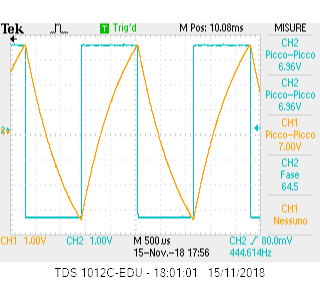
\includegraphics[scale=0.8]{v+_v-.png}
		\caption{\small i segnali $V_+$( in azzurro ) e $ V_-$ ( in arancione )  multivibratore astabile}

		\label{fig:v+v-}
	\end{center}

\end{figure}



\begin{figure}[h]
	\begin{center}
		
			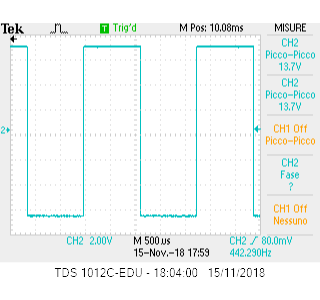
\includegraphics[scale=0.8]{vout_punto2.png}
		\caption{\small segnale $V_{out}$ del multivibratore astabile }

		\label{fig:v+v-}
	\end{center}

\end{figure}


d) La serie di  diodi  Zener limita l'escursione in tensione, infatti deve essere $|V_{out}| \le V_{\gamma} +V_{z} = V_{Max}$.
 Se $V_{1}$ (segnale all'uscita dell'Op-Amp) fosse maggiore dii $V_{max}$ si avrebbe un cortocircuito; per evitare questa eventualità si introduce  una resistenza $R_3$ che limita la corrente.

\rem{mettere ddp morse}





\end{document}          
